%% 
%% Introduction
%%
%% Key ideas: 
%%
%% 1. Augmenting feature models with application domain modeling
%% 2. Impact this has on the toolsuite for featureIDE and composition engines
%%
%% 3. Expose programming API instead of providing a standard black-box
%%    capability, which might otherwise restrict users' abilities.

Software product lines (SPLs) refer to software engineering methods,
tools and techniques for creating a collection of similar software
systems, called product line members, from a shared set of software
assets using a common means of production. A number of characteristics
separate SPLs from routine large, complex systems and thus there is a need for specialized tools and techniques to design, implement and maintain SPLs. 

Fundamental to many SPL approaches is the concept of a \textit{Feature
Model}, first introduced by the Feature-Oriented Domain Analysis (FODA)
technique~\cite{Kang1990} and refined over the years by numerous
researchers. A feature model is composed of user-visible features from
which a wide variety of configurations can be defined through the
selection of individual features. Many tool chains have been developed
to generate product line members ``on demand'' from a feature model
configuration. Developers need to construct the SPL code artifacts in a
specific way that enables the tools to work; this may include, for
example, low-level compiler directives embedded in source code, or
specialized languages (such as JAK~\cite{Batory2004FeatureorientedPA} or
DeltaJ~\cite{Schaefer:2010:DPS:1885639.1885647}) that developers use to
encode the artifacts.

%%\begin{figure}
%%    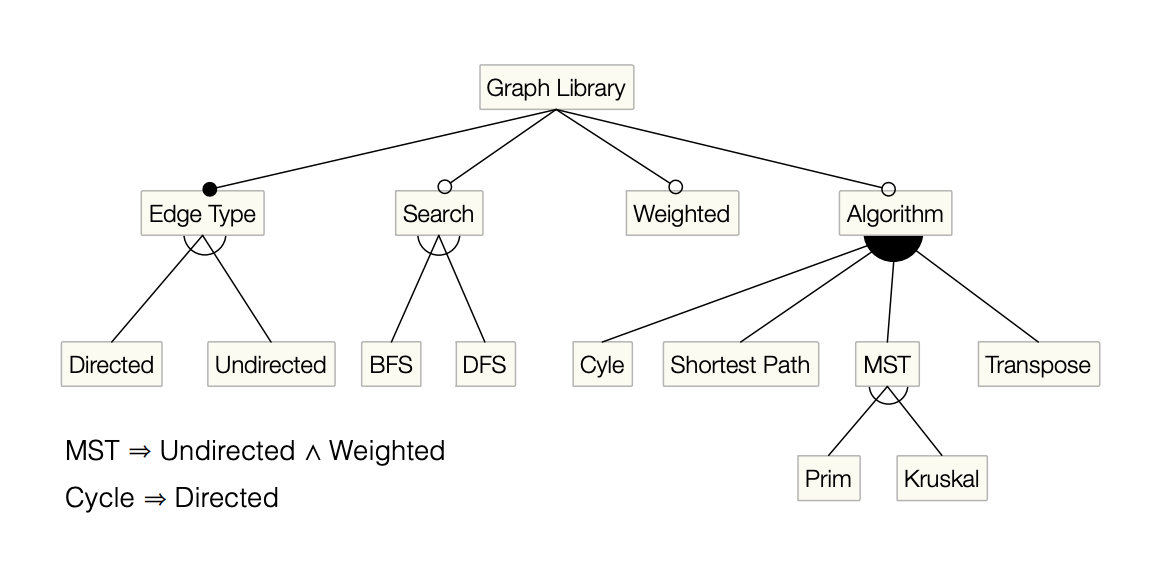
\includegraphics[scale=0.4,natwidth=1154,natheight=576]{gpl2.png}
%%    \caption{Graph Product Line Feature Model}
%%    \label{fig:feature-model}
%%\end{figure}

There remains a potential issue, however, when the variability inherent in the product line relates to the application domain model. The common result is that one must integrate these domain-model concepts into the feature model so they can become part of the configuration process. The feature model from Figure~\ref{fig:feature-model} contains features relating to behavior (i.e., \textbf{Prim} contains Prim's implementation of the Minimum Spanning Tree problem) and some relate to structure (i.e., \textbf{Weighted} captures the notion that edges in a graph may have weights). 

In past work, we have explored product lines within a number of application domains~\cite{Heineman:2015:TMO:2791060.2791076,PEPM18}

%We make the following observations regarding product lines:
%
%--
%
%--Should be able to add to and remove features from a product line after it has been defined
%
%--A product line definition is still reflected in software artifacts, which means it should support common refactoring functionality
%
%--Should be feature-rich, which means one can potentially envision a significant number of PL members (e.g., not just a handful)
%
%Without one of these characteristics, it could only be considered a closed system.


% A SPL is a family of related programs. When the units of program
% construction are feature—increments in program functionality or
%development—every program in an SPL is identified by a unique and legal
%combination of features, and vice versa. Family member refers to
%individual product. A variation point represents a decision leading to
%different variants of an asset. A variation point consists of a set of
%possible instantiations (legal variations of the variation point). A
%variation point usually specifies the binding times, that is the
%time/times at which a decision about the instantiation has to be taken.

%The variant derivation is the action in which assets are combined from
%the set of available assets and contained variation points are
%bound/instantiated. If there are variation points with multiple binding
%times, the derivation will happen stepwise at each binding time. The
%result of such a derivation is a set of derived assets. The derivation
%can be executed technically in many ways. The simplest way is to copy
%assets and modify (parts of) them (e.g. the configuration parameters)
%manually. The result of such a derivation is often called a
%configuration.



%% THESE NEED TO BE PLACED IN CONTEXT.
Here is a reference to K\"{a}stner's paper~\cite{Kastner:2012}.

Here is a reference to ~\cite{leich2005tool}.
Here is a reference to ~\cite{proksch2014tool}.
Here is a reference to ~\cite{7203038}.
Here is a reference to ~\cite{Sayre:2005:UMA:1082983.1083277}.
Here is a reference to ~\cite{Setyautami:2016:UPD:2934466.2934479}.
Here is a reference to ~\cite{Sousa:2016:EFM:2934466.2934475}.

Here is a reference to ~\cite{Arcaini:2017:ARV:3106195.3106206}.

Here is a reference to ~\cite{Vasilevskiy:2016:TRP:2934466.2934484}.

Here is a reference to ~\cite{Kuhn:2015:CPC:2791060.2791092}.

Here is a reference to ~\cite{Schaefer:2010:DPS:1885639.1885647}.

Here is a reference to ~\cite{Apel:2008:AFF:1428476.1428480}.


\subsection{Approaches to Product Line Development}

Software product lines create unique engineering challenges for a number
of reasons. First, it should be possible to generate any number of
instances of the product line, and by this we mean the code artifacts
for the instance application. These are then compiled (or interpreted)
to realize the execution of the application. Second, there are multiple
development efforts; one can work on code that will effectively be used
by all product line instances, but at other times, one is focused on
writing code for just a single instance from the PL.

A major goal of featured-oriented PL is to derive a product
automatically based on user’s selection. There are three philosophical
approaches widely used in practice -- \textit{annotation-based} ,
\textit{composition-based} or \textit{component-based} -- which differ in the way they represent
variability in the code base and the way they generate products.

\subsubsection{Annotation-based Approach}

There is a single body of code artifacts which fully contains all code
resources used by all members of the product line. Using different tools
or language-specific capabilities, a compiler (or processor) will
extract subsets of the code to be used for a PL instance. One of the
most common approaches is to use compiler directives embedded within the
code as a means for isolating code unique to a subset of product line
instances. Then each product line instance can be generated by compiling
the same code base with different compiler flags, resulting in different
executable instances. Due to the nature of this approach, often one
cannot review the source code for individual
instances.~\cite{Apel:2013:FSP:2541773}.

In annotation-based approaches, the code of all features is merged in a single code base, and annotation mark which code
 belongs to which feature. In some sense, an annotation is a function that maps a program element to the feature or
 feature combination it belongs to.

Annotation-based approaches are widely used in practice because they are easy to use and already natively supported
by many programming environments. It keeps good readability and low complexity, however, relatively simple tool support
can address scattered code or error.

~cite{Kastner:2012,Apel:2013:FSP:2541773,Arcaini:2017:ARV:3106195.3106206,Liebig:2013:SAV:2491411.2491437}



\subsubsection{Composition-based Approach}

Another approach is to design a feature tree which is used to capture all the externally visible features that
can be used to differentiated one product line instance from another. Then code assets are internally associated
 with each of these visible features. Finally product line instances are configured by selecting for inclusion
  features from the feature tree, potentially restricted by constraints. A composition engine processes the
  code assets associated with the selected features to create the final source code for the product line instance.

Composition-based approaches locate code belonging to a feature or feature combination in a dedicated file,
container, or module. A classic example is a framework that can be extended with plug-ins, ideally one plug-in
per feature. The key challenge of composition-based approaches is to keep the mapping between features and
composition units simple and tractable.

Another way to view the difference between annotation and composition is that annotation separate concerns
virtually and composition separate concerns physically,and code is removed on demand with annotation while
composition units are added on demand.

~\cite{Thum:2014:FEF:2537169.2537315,Apel:2013:FSP:2541773,Schaefer:2010:DPS:1885639.1885647
,Dhungana:2011:DMD:1924082.1924092,Heineman:2015:TMO:2791060.2791076,Batory2004FeatureorientedPA,
leich2005tool,Setyautami:2016:UPD:2934466.2934479,Ddder2013UsingII,Apel:2009:FLA:1555001.1555038,
proksch2014tool}.

\subsubsection{Component-based Approach}

A software component is a unit of composition with contractually specified interfaces and explicit context
dependencies only. A software component can be deployed independently and is subject to composition by third
parties. The key idea of a component is to form a modular, reusable unit.

Developing product line by constructing and composing reusable was a common strategy. With domain analysis,
developers decided which functionality should be reused across multiple products of the product line designed
components accordingly. To derive a product for a given feature selection during application engineering, a
developer selects suitable components and then manually writes glue code to connect components for every
product individually.

~cite{Kuhn:2015:CPC:2791060.2791092,atkinson2000component}.


\subsubsection{Product Line Techniques In Industry}

Annotation-based approach are not so widely used as composition-based approach because drawbacks mentioned above.
Here are some existing annotation-based approaches:

code coloring (FeatureCIDE): CIDE is an Eclipse plug-in that replaces the Java editor in SPL projects. Developers
start with a standard Java legacy application, then they select code fragment and associate them with features
 from the context menu. The marked code is then permanently highlighted in the editor using a background color
 associated with the feature. Here is a reference to ~\cite{CIDE:Eclipse}.


Type checking approach,  a product-line-aware type system that statically and efficiently detects type errors in
annotation-based product-line implementations.~\cite{Kastner:2012}


To work with FeatureIDE, the primary challenge is to design a feature tree model to represent the desired product
line application domain. Because features are cross-cutting with regards to the artifacts in the programming
language, the various composer engines supported by FeatureIDE accomplish the same goal in a variety of ways.

AHEAD has feature modules for each concrete feature, and the corresponding composition tool places generated
source code directly into the Eclipse source folder. AHEAD brings separate tools together and selects different
tools for different kinds of files during feature composition,establishing a clear interface to the build
system. Composing Jak files will invoke a Jak-composition, whereas composing XML files invokes an
XML-composition tool.~\cite{Batory2004FeatureorientedPA}.

FeatureHouse tool suite has been developed that allows programmers to enhance given languages rapidly with
support for feature-oriented programming. It is a framework for software composition supported by a
corresponding tool chain. It provides facilities for feature  composition based on a language-independent
model and tool chain for software artifact, and a plug-in mechanism for the integration of new artifact
languages.~\cite{Apel:2009:FLA:1555001.1555038}

Deltaj is a Java-like language which allows to organize classes in modules. A program consists of a base
 module and a set of delta module in a stepwise manner. Much like a feature module, a delta module can add
 new classes and members as well as extend existing methods by overriding. In contrast to feature modules,
 delta modules can also delete existing classes and individual members.~\cite{Schaefer:2010:DPS:1885639.1885647}.

In LaunchPad, each feature can contain any number of combinators, designed using a DSL we had developed to
simplify the writing of combinators for an earlier CLS tool. A configuration is a subset of features from
which a repository is constructed. Each feature can optionally store target definitions, which are aggregated
 together and then used as the basis for the inhabitation requests, i.e.As each request is satisfied, the
 synthesized code from the resulting type expression M is stored in the designated source folder.
~\cite{Heineman:2015:TMO:2791060.2791076}.

\subsubsection{Evaluation of related work}

The key challenge of composition-based approaches is to keep the mapping between features and composition units
simple and tractable. Preprocessor-based and parameter-based implementations are often criticized for their
potential complexity, lack of modularity, and reduced readability. And they all have some problems which is the
difficulty to refactoring.~\cite{Kim:2017:RJS:3106195.3106201}.

Although component-based implementations are common in product line practice, they lack the automation potential
of feature orientation that we aim at. Deciding when to build a reusable component and what to include in
that component is a difficult design decision, one need to have good understanding of whole scope to do that.
There is no domain in this approach, glue code is a necessary, it's no more than assembling components.
~\cite{Apel:2013:FSP:2541773}

In practice most PLs appear “from the ground up” where developers take advantage of language-specific capabilities
 to annotate different code regions as being enabled (or disabled) based on compiler directives. Starting from an
 annotation-based code repository many composition-based approaches simply “snipped” or refactored code fragments
 to recreate countless tiny “features” that could be selected.

Manual composition is a configuration process. A designer selects individual features from a feature model and
relies on constraints to ensure the resulting product line member is valid. Manual Composition is limited to a
potential total of 2N configurations where N represents the number of available features in the model. There is no
 domain modeling, What commonly occurs is the designer must make sure that changes to any of the units will not invalidate those product
 line members that incorporate that feature.

 Another problem is that the features are fixed and unchanging. If we need to make some modifications to current
 instances, we may need to trace all the way back and change the code in many classes because it’s inheritance
 structure. If we want to add features which is slightly different from existing ones, we may need to start from
 very beginning.
